% additional use of \usepackage{beamerthemesplit}
\documentclass{beamer}
\usepackage{beamerthemesplit} % new 
\usepackage{hyperref}
\usepackage{multimedia}
\usepackage{animate}
\usepackage[export]{adjustbox}


\definecolor{verde}{rgb}{0.5,1,0.2}
\definecolor{rojo}{rgb}{1,0,0}
\definecolor{azul}{rgb}{0,0,1}

\begin{document}

\title{Machine Learning techniques applied to cosmological problems.} 
\author{Mart\'in de los Rios} 
\date{}

\frame{
  \titlepage
  Director: Dr. Mariano Dom\'inguez
} 

\frame{
  \tiny
  \frametitle{Resumen}
  \tableofcontents
} 

\section{Introduction to Machine Learning techniques.}

\frame{
\tableofcontents[ 
    currentsubsection, 
    sectionstyle=show/hide, 
    sectionstyle=show/shaded, 
    ] 
}

\frame{
  \frametitle{Supervised Learning.}
  \begin{center}
   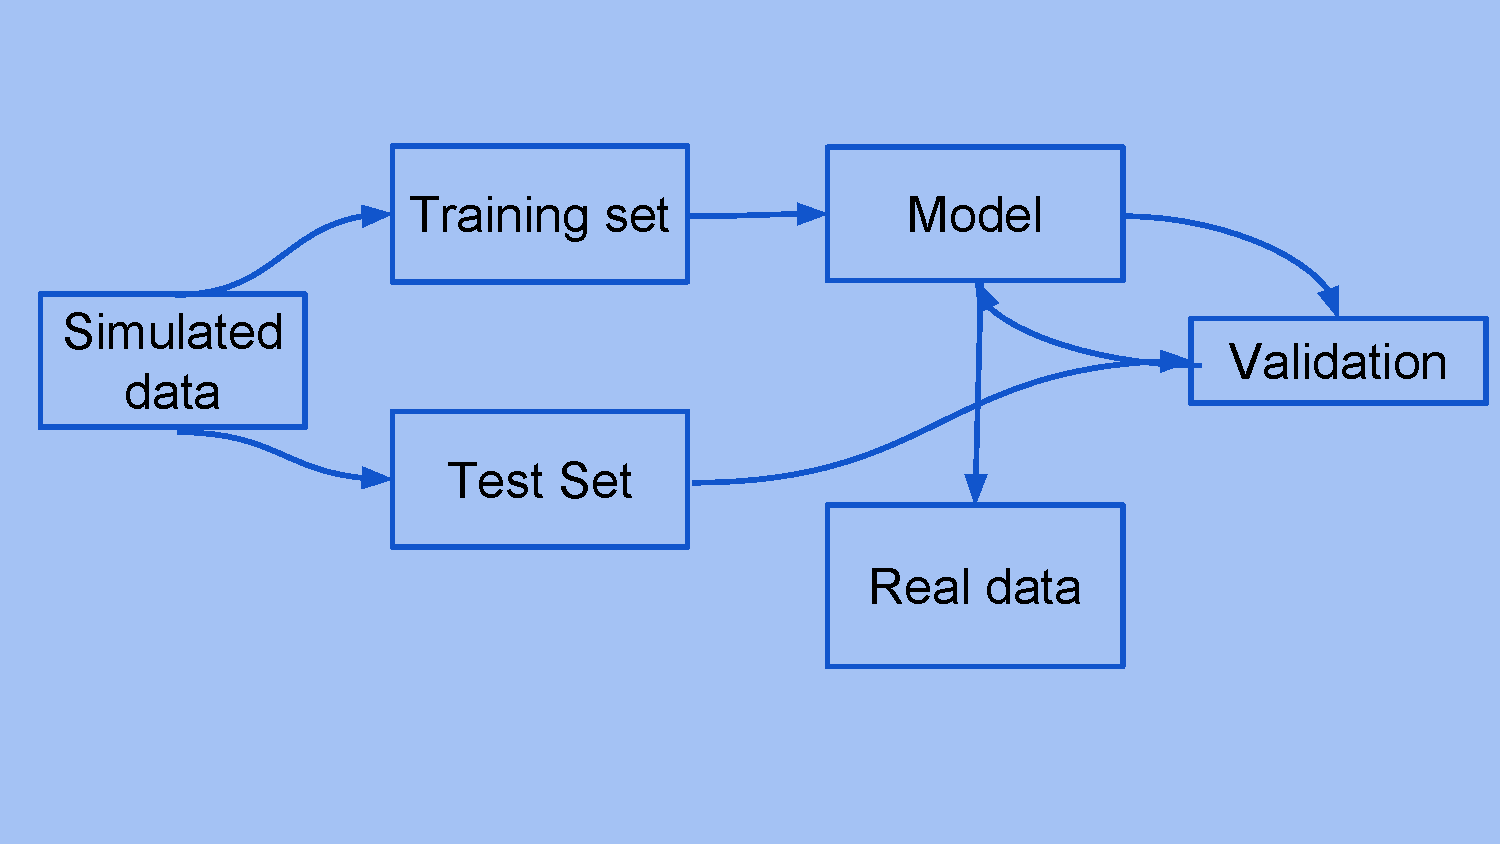
\includegraphics[scale=0.45]{./aprendizaje_supervisado.pdf}
  \end{center}
}

\begin{frame}{Random Forest}
\begin{center}
  \animategraphics[loop,controls,scale=0.5]{10}{random_forest-}{0}{20}
\end{center}
\end{frame}

%\frame{
%  \frametitle{Random Forest}
%  \begin{center}
% 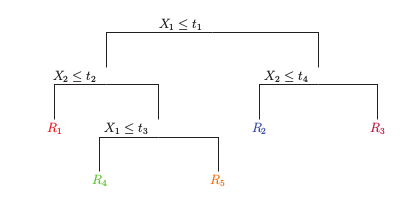
\includegraphics[scale=0.85]{./rf.png}
 % rf.png: 0x0 pixel, 300dpi, 0.00x0.00 cm, bb=
%\end{center}

%}

\begin{frame}{Support Vector Machines}
\begin{center}
  \animategraphics[loop,controls,scale=0.3]{10}{support_vector_machines-}{0}{40}
\end{center}
\end{frame}

%\frame{
%  \frametitle{Support Vector Machine}
%  \begin{center}
% 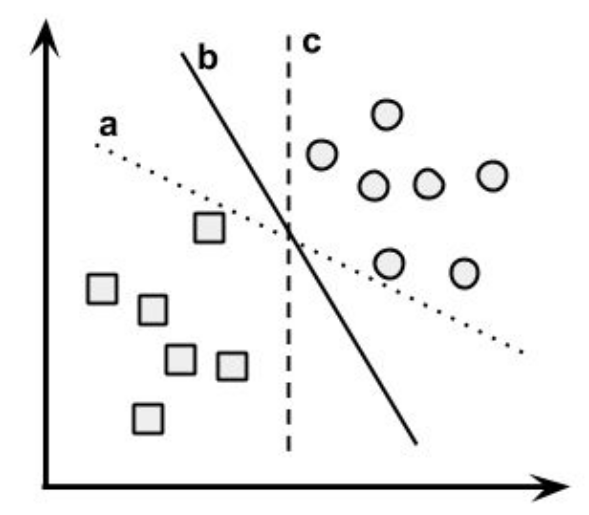
\includegraphics[scale=0.4]{./svm.png}

 % svm.png: 0x0 pixel, 300dpi, 0.00x0.00 cm, bb=
%\end{center}
%}

\frame{
  \frametitle{Unsupervised Learning.}
  \begin{center}
 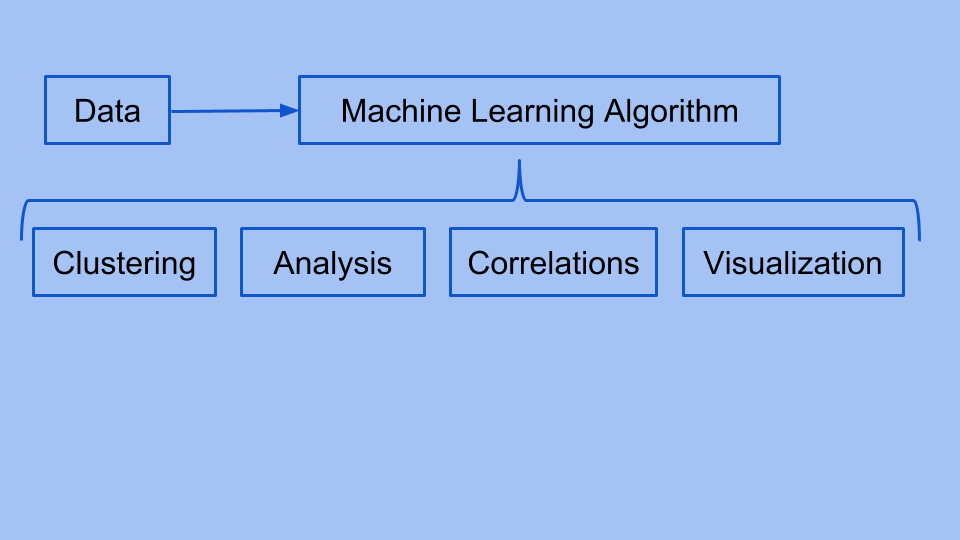
\includegraphics[scale=0.34]{./aprendizaje_nosupervisado.png}
 % aprendizaje_nosupervisado.jpg: 0x0 pixel, 300dpi, 0.00x0.00 cm, bb=
\end{center}

}

\begin{frame}{Mixture of Gaussians}
\begin{center}
  \animategraphics[loop,controls,scale=0.5]{10}{mixture_of_gaussians-}{0}{14}
\end{center}
\end{frame}

%\frame{
% \frametitle{Mixture of Gaussians.}
% \begin{center}
% 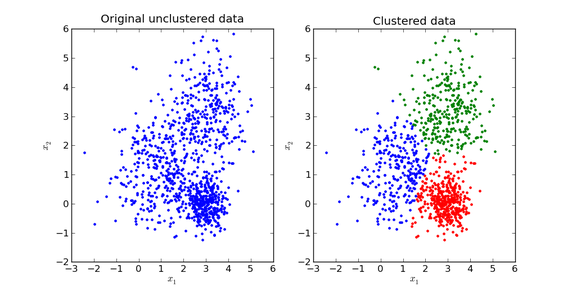
\includegraphics[scale=0.5]{./mixt_gauss.png}
 % mixt_gauss.png: 0x0 pixel, 300dpi, 0.00x0.00 cm, bb=
%\end{center}
%}

\frame{
\frametitle{Principal Components Analysis.}
\begin{center}
 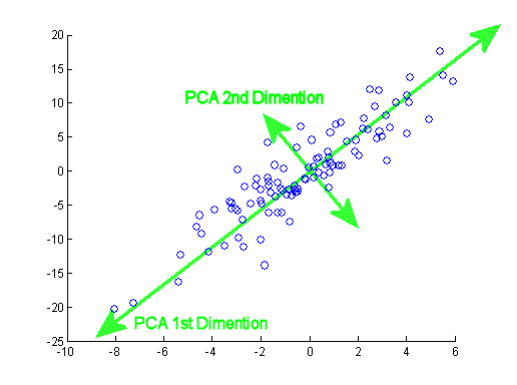
\includegraphics[scale=0.5]{./pca.png}
 % pca_example.gif: 0x0 pixel, 300dpi, 0.00x0.00 cm, bb=
\end{center}

}

\section{The \texttt{MeSsI} (Merging Systems Identification) Algorithm.}

\frame{
\tableofcontents[ 
    currentsubsection, 
    sectionstyle=show/hide, 
    sectionstyle=show/shaded, 
    ] 
}
\frame{
\begin{figure}[ht!]
 \centering
 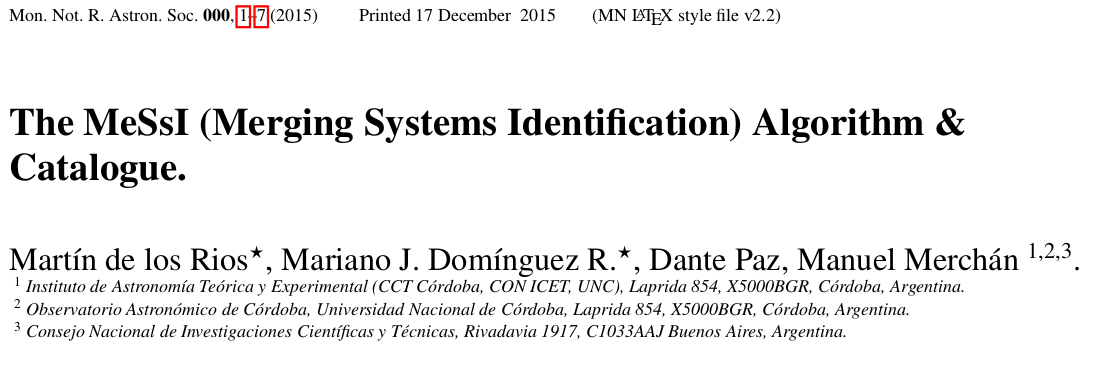
\includegraphics[scale=0.45]{messi_paper.png}
 % messi_paper.png: 1020x278 px, 72dpi, 35.98x9.81 cm, bb=0 0 1020 278
\end{figure}

}
\frame{
\begin{figure}[ht!]
 \centering
 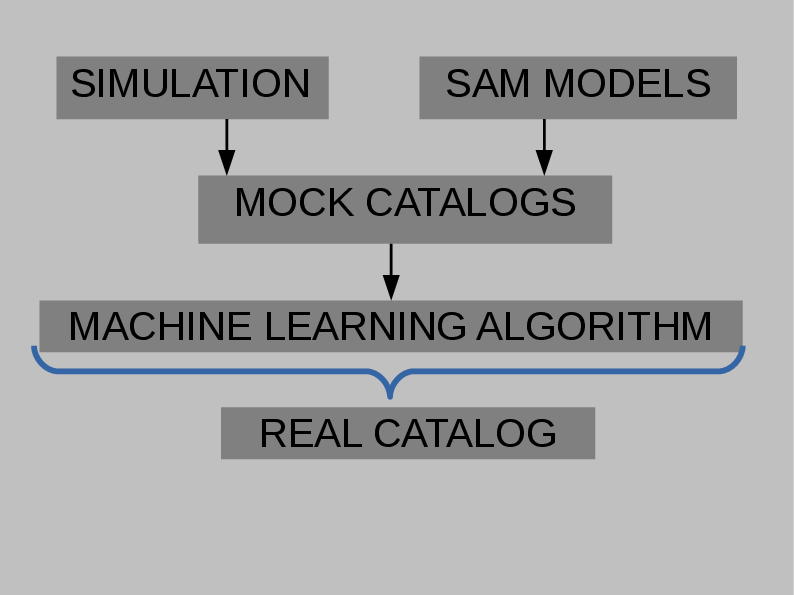
\includegraphics[scale=0.35]{resu.png}
 % resu.png: 794x595 px, 72dpi, 28.01x20.99 cm, bb=0 0 794 595
\end{figure}
}
\frame{\frametitle{Study of the merger trees.}
 \begin{itemize}
  \item Based on the subhalos merger trees, we construct the merger tree for every fof group in the simulation.
 \end{itemize}
 \begin{figure}[h!]
  \centering
  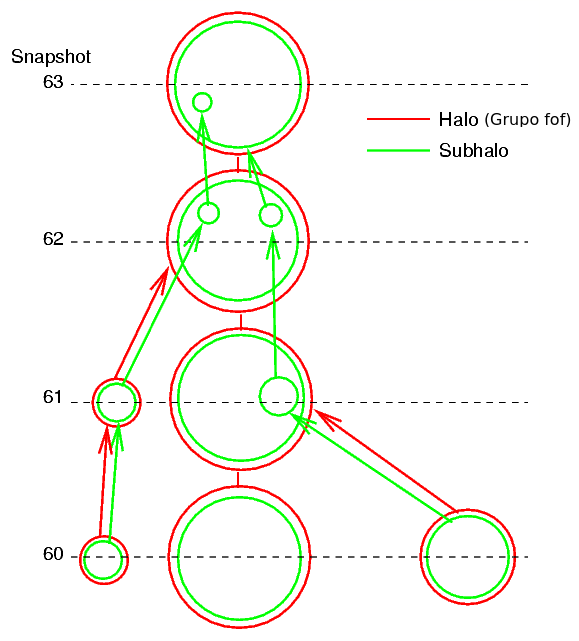
\includegraphics[scale=0.32]{./tree.png}
 % tree.eps: 0x0 pixel, 300dpi, 0.00x0.00 cm, bb=14 14 554 655
 \end{figure}
}
\frame{
 \begin{columns}
  \begin{column}{5cm}
   \begin{itemize}
    \item Dressler-Shectman test.
    \item Non gaussianity test.
    \item Color.
    \item Number of galaxies.
   \end{itemize}
  \end{column}
  \begin{column}{5cm}
   \begin{figure}[h!]
    \centering
    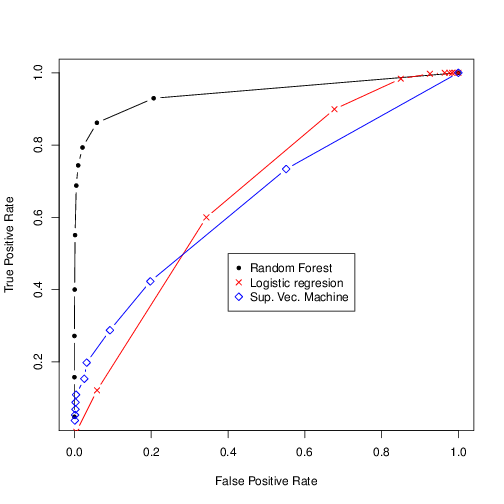
\includegraphics[scale=0.35]{./roc_curves.png}
    % roc_curves.pdf: 504x504 pixel, 72dpi, 17.78x17.78 cm, bb=0 0 504 504
   \end{figure}
  \end{column}
 \end{columns}
}
\frame{
\begin{itemize}
 \item We found $61$ candidates to merging clusters.
 \item In $32$ of these we were able to identify the colliding substructures.
 \item $21$ of these were previously classified as merging clusters by other authors.
\end{itemize}

\begin{figure}[ht!]
 \centering
 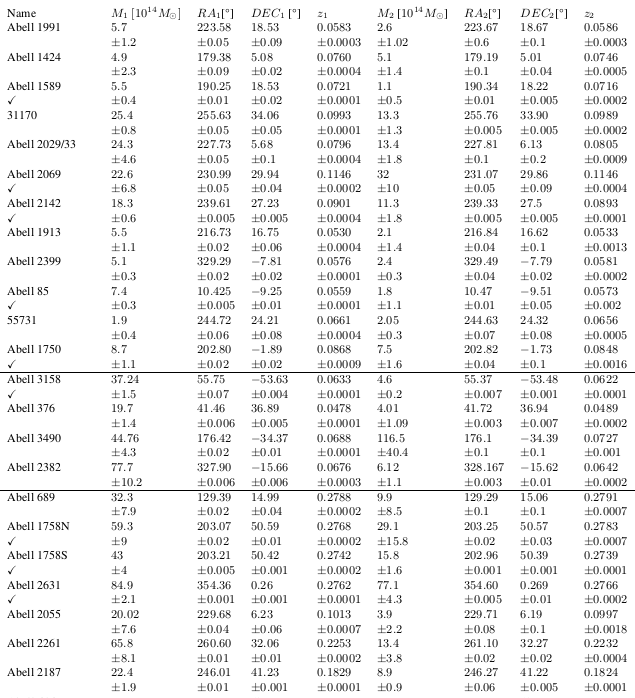
\includegraphics[scale=0.3]{conclusiones_messi.png}
 % conclusiones_messi.png: 635x698 px, 72dpi, 22.40x24.62 cm, bb=0 0 635 698
\end{figure}
}
\section{Analysis of individual merging clusters candidates.}

\frame{
\tableofcontents[ 
    currentsubsection, 
    sectionstyle=show/hide, 
    sectionstyle=show/shaded, 
    ] 
}
\frame{
\begin{figure}[ht!]
 \centering
 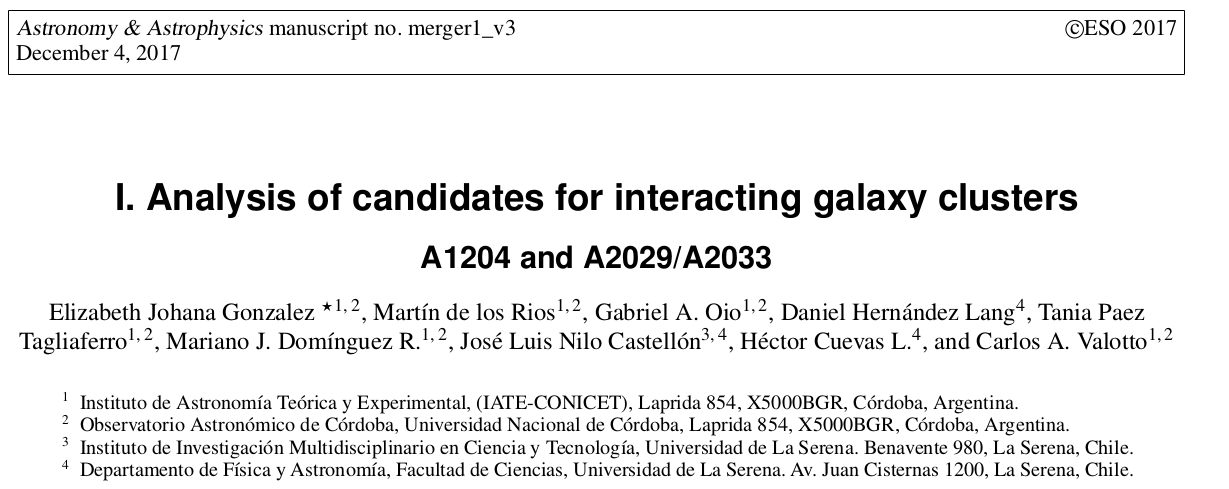
\includegraphics[scale=0.38]{a2029_paper.png}
 % a2029_paper.png: 1094x200 px, 96dpi, 28.94x5.29 cm, bb=0 0 820 150
\end{figure}
}

\subsection{A2029/2033.}
\frame{
\begin{figure}[ht!]
 \centering
 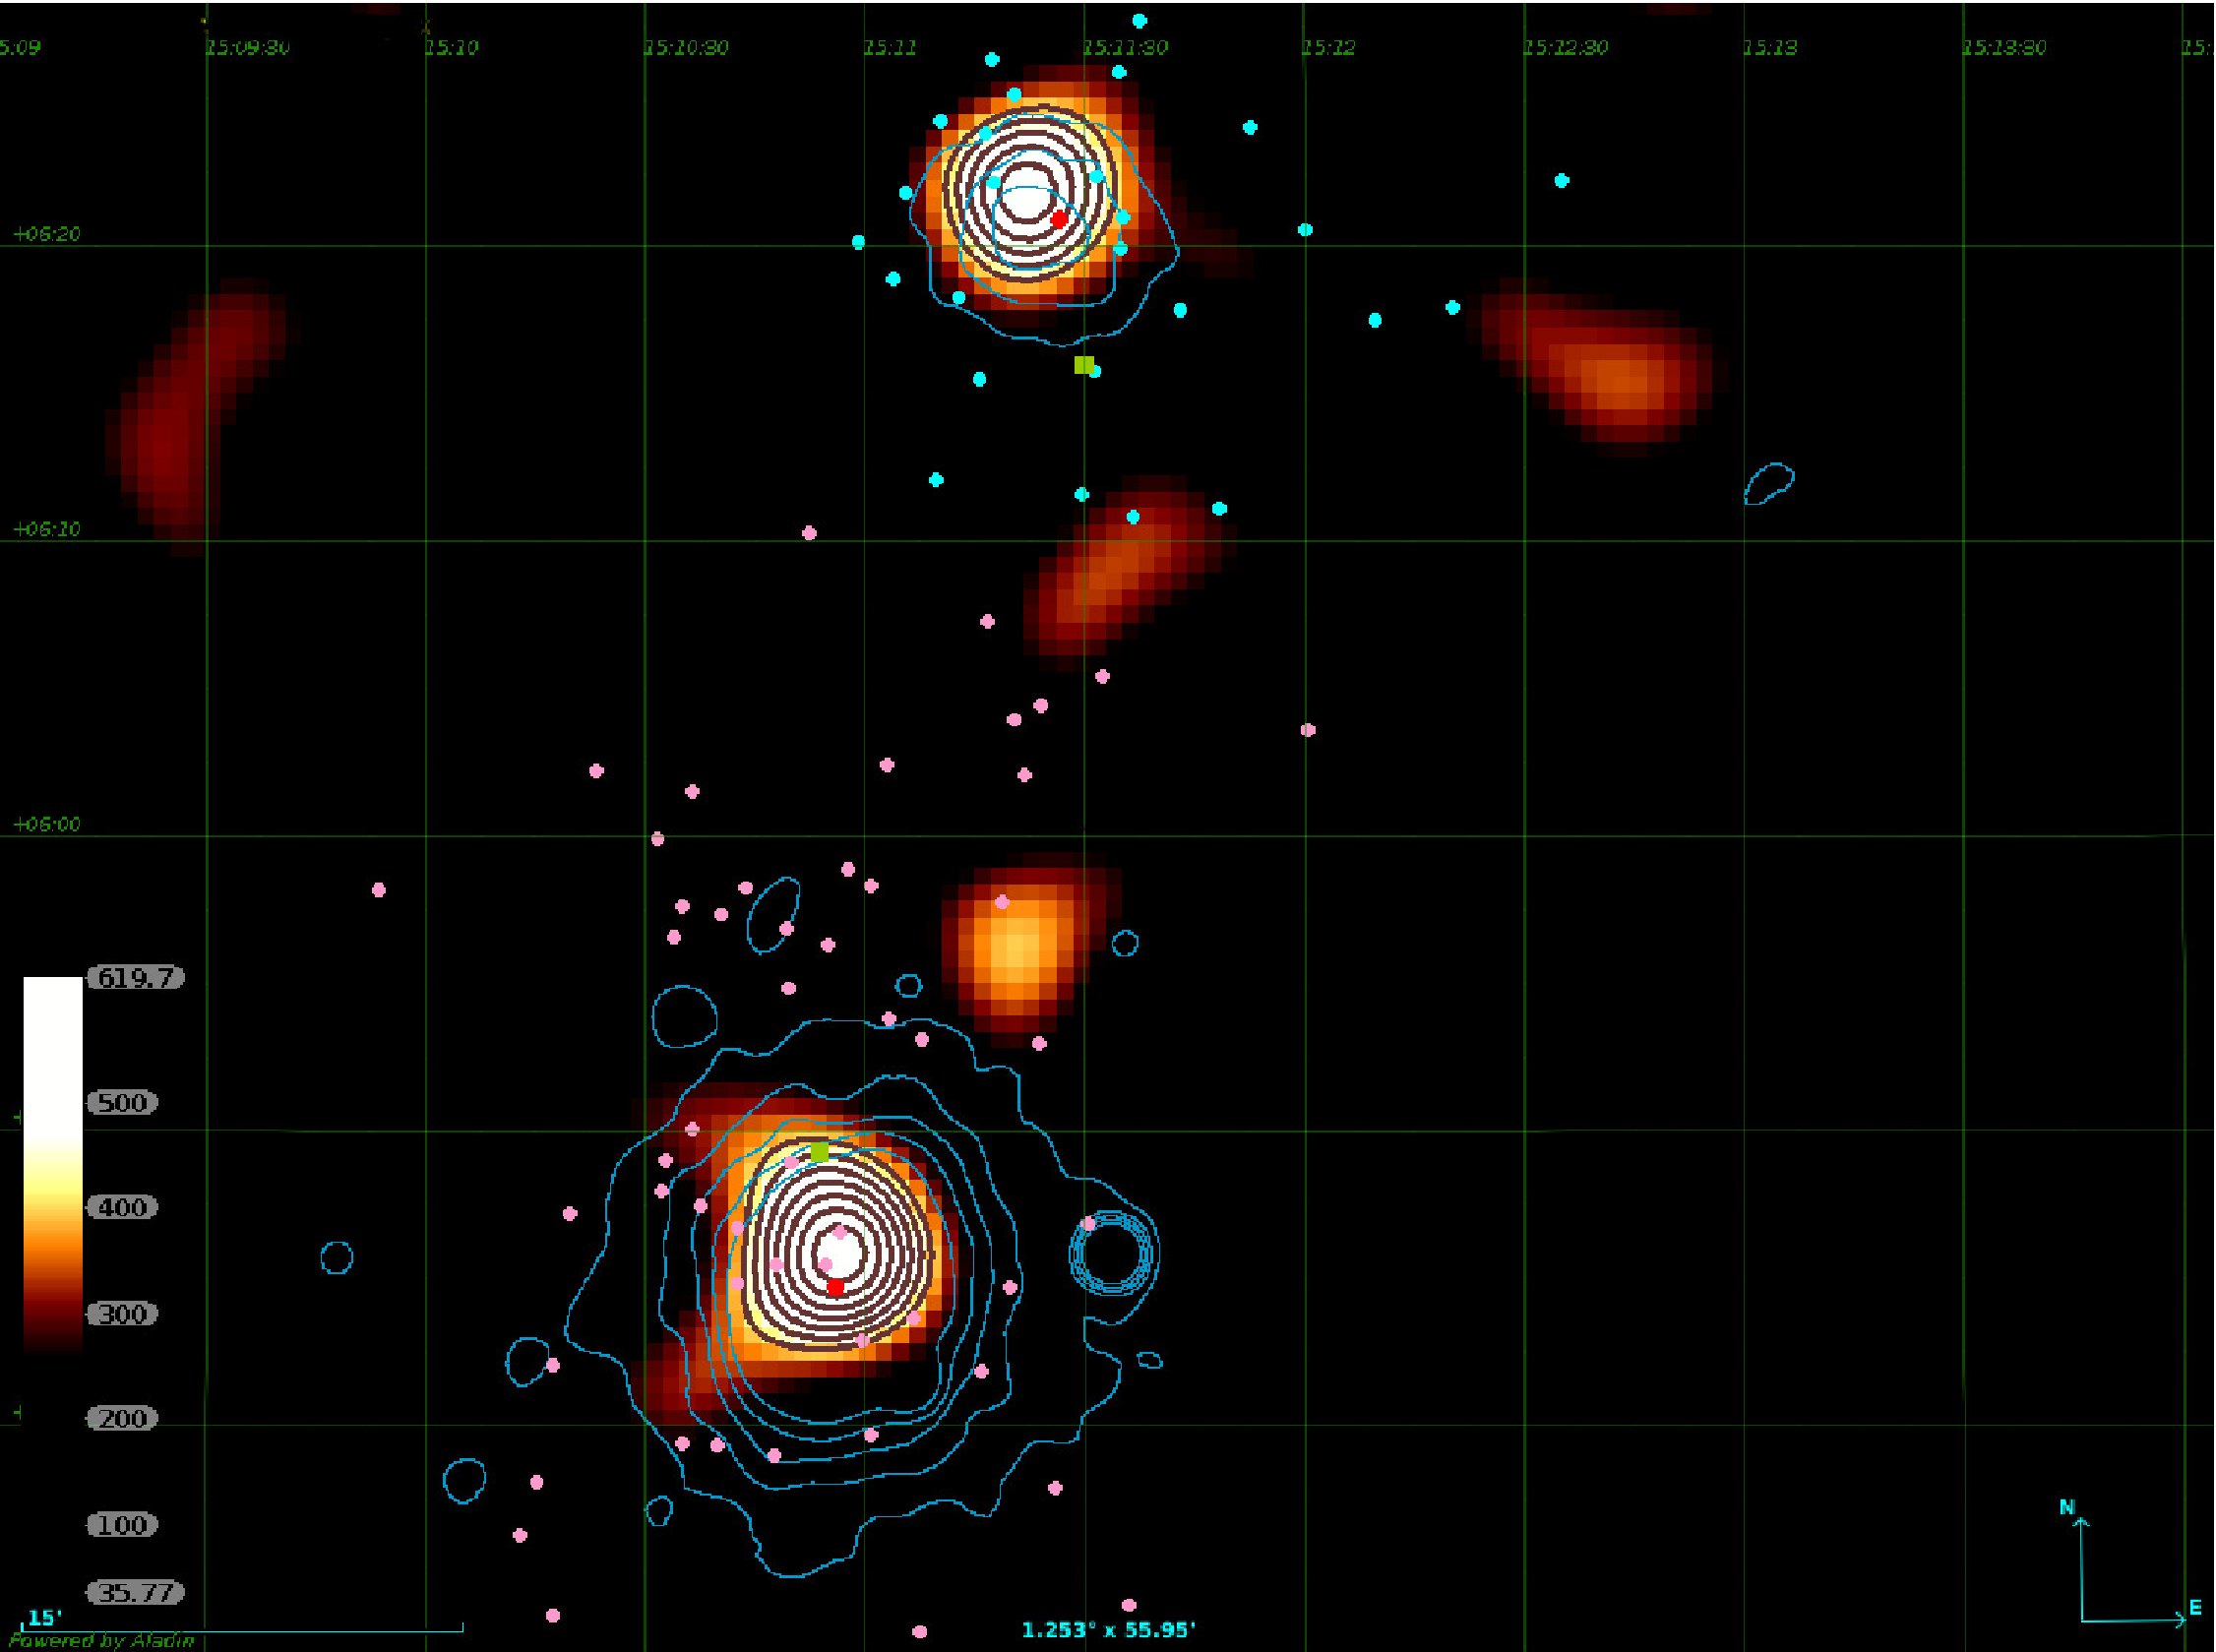
\includegraphics[scale=0.25]{A2029-2033-eps-converted-to.pdf}
 % A2029-2033-eps-converted-to.pdf: 0x0 px, 300dpi, 0.00x0.00 cm, bb=
\end{figure}

}
\subsection{A1204.}
\frame{
\begin{figure}[ht!]
 \centering
 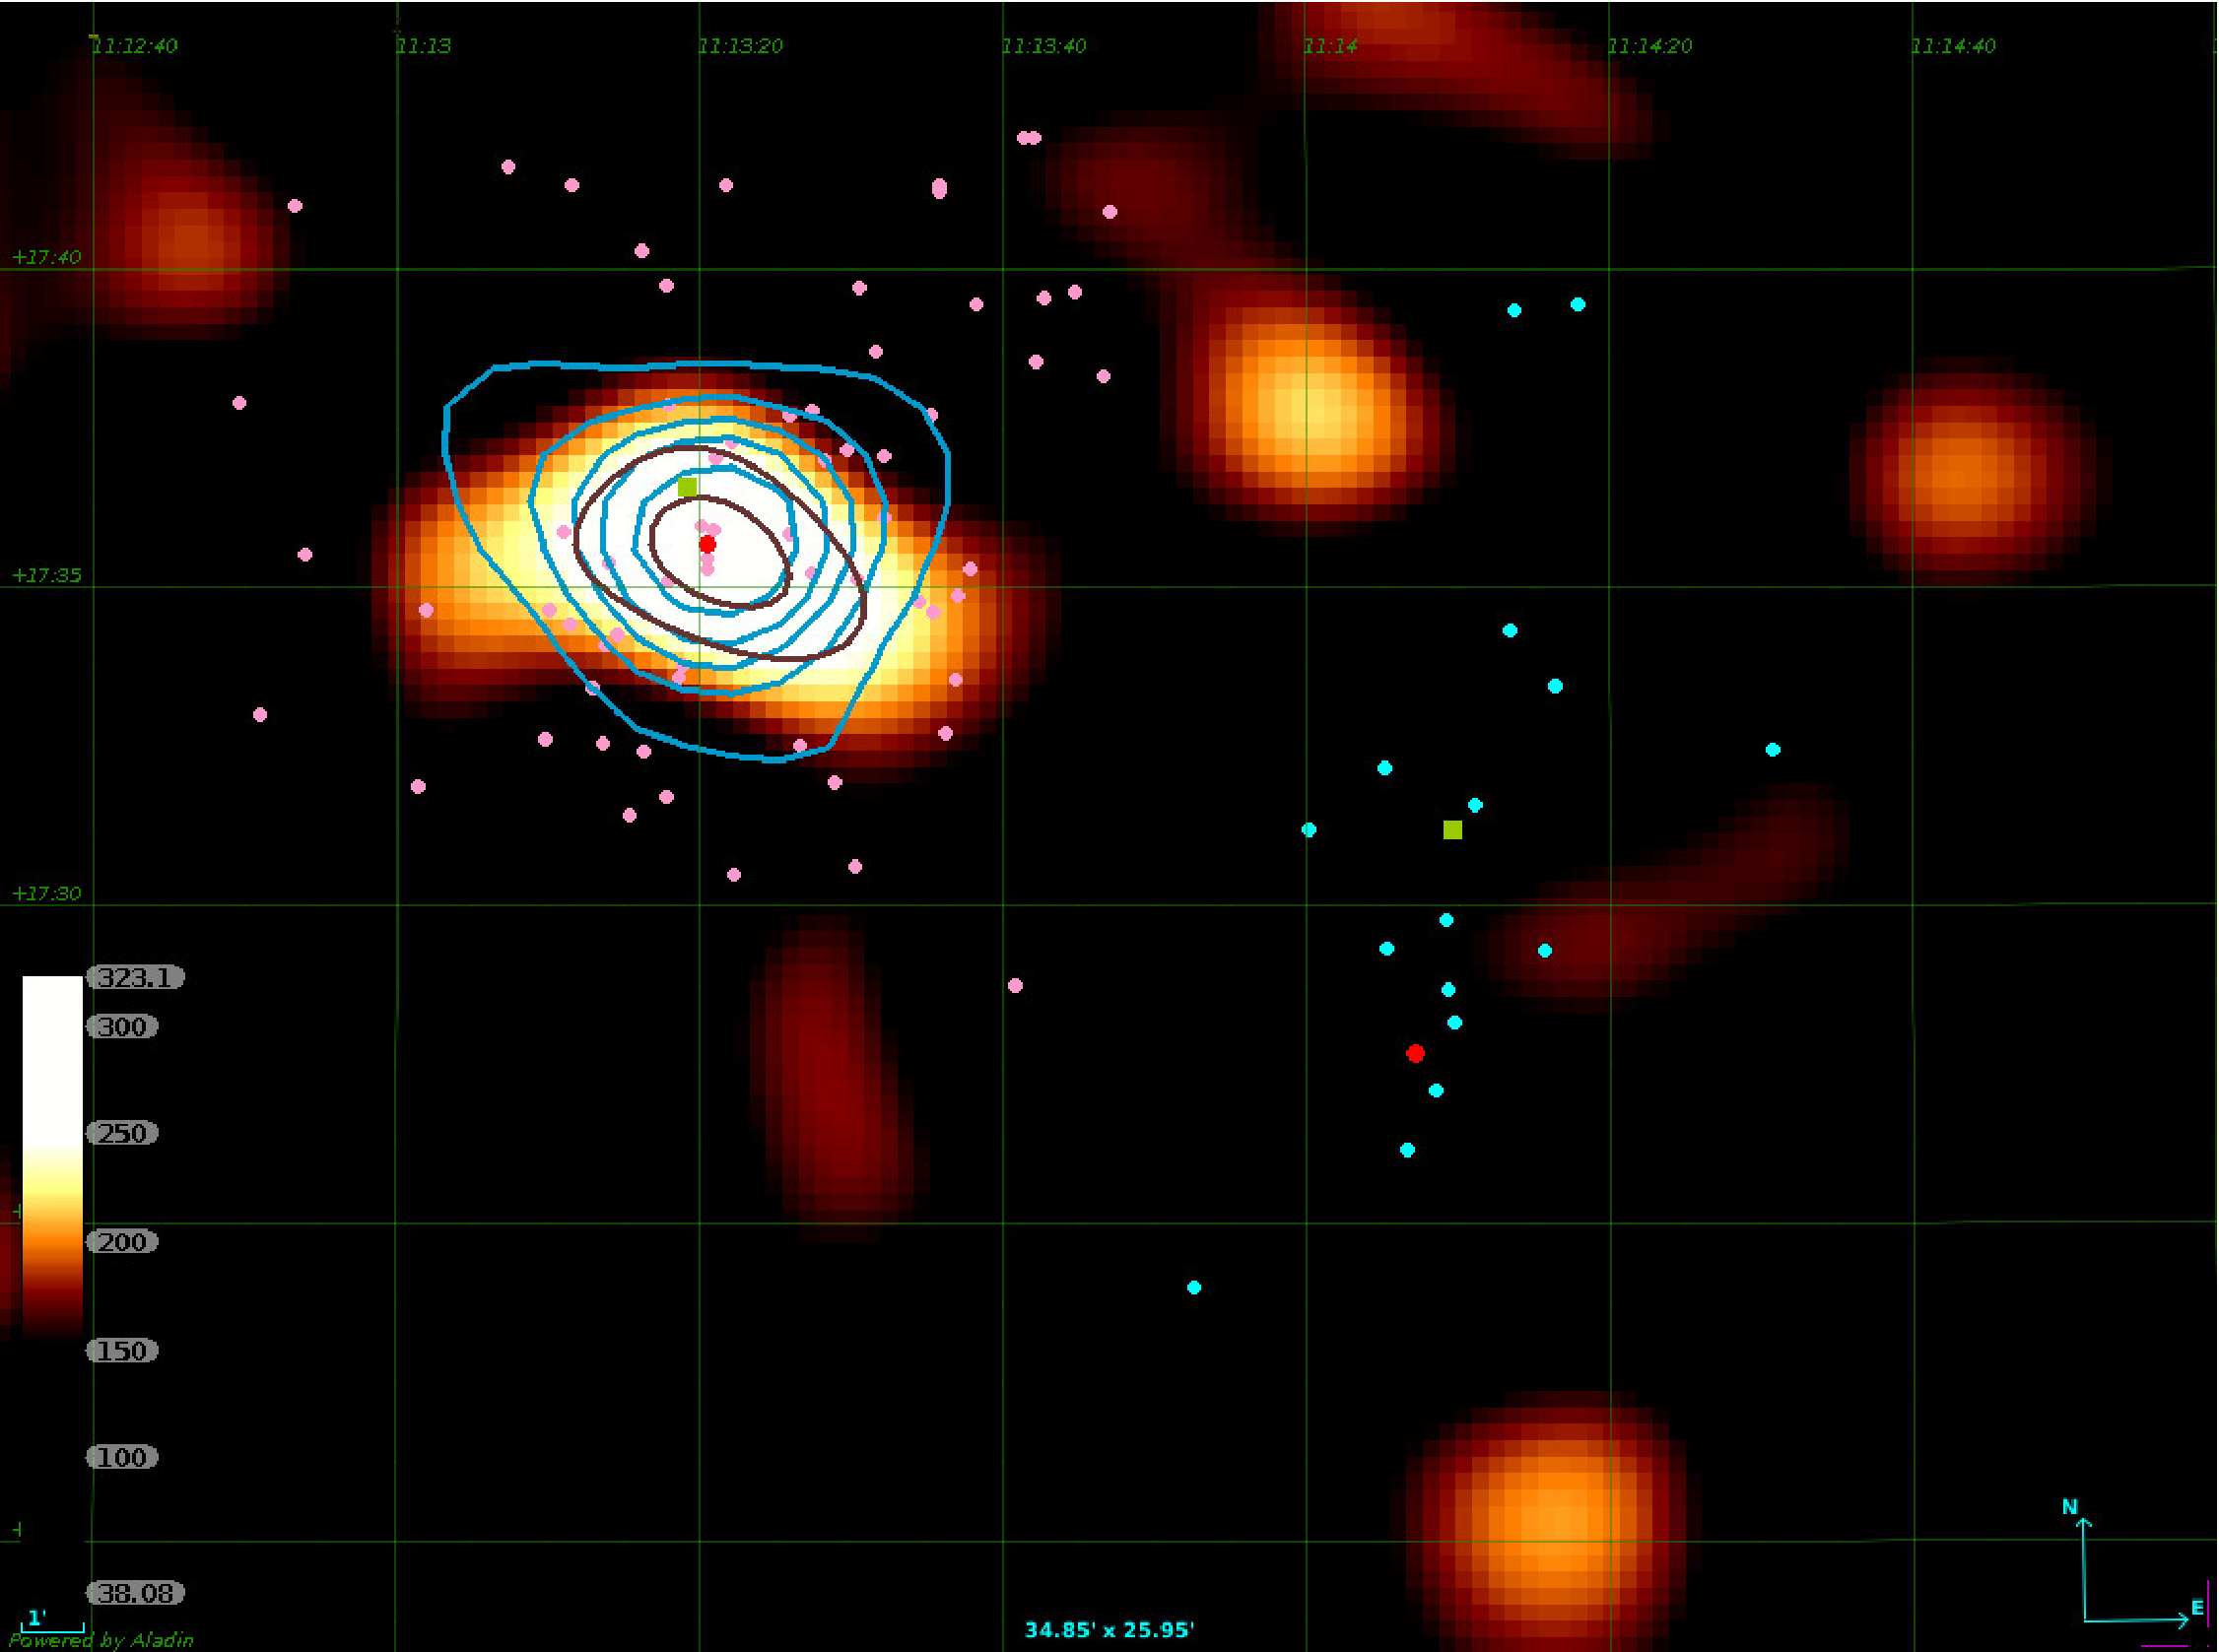
\includegraphics[scale=0.25]{A1204-eps-converted-to.pdf}
 % A1204-eps-converted-to.pdf: 0x0 px, 300dpi, 0.00x0.00 cm, bb=
\end{figure}
}
\subsection{A267.}
\frame{
\begin{figure}[ht!]
 \centering
 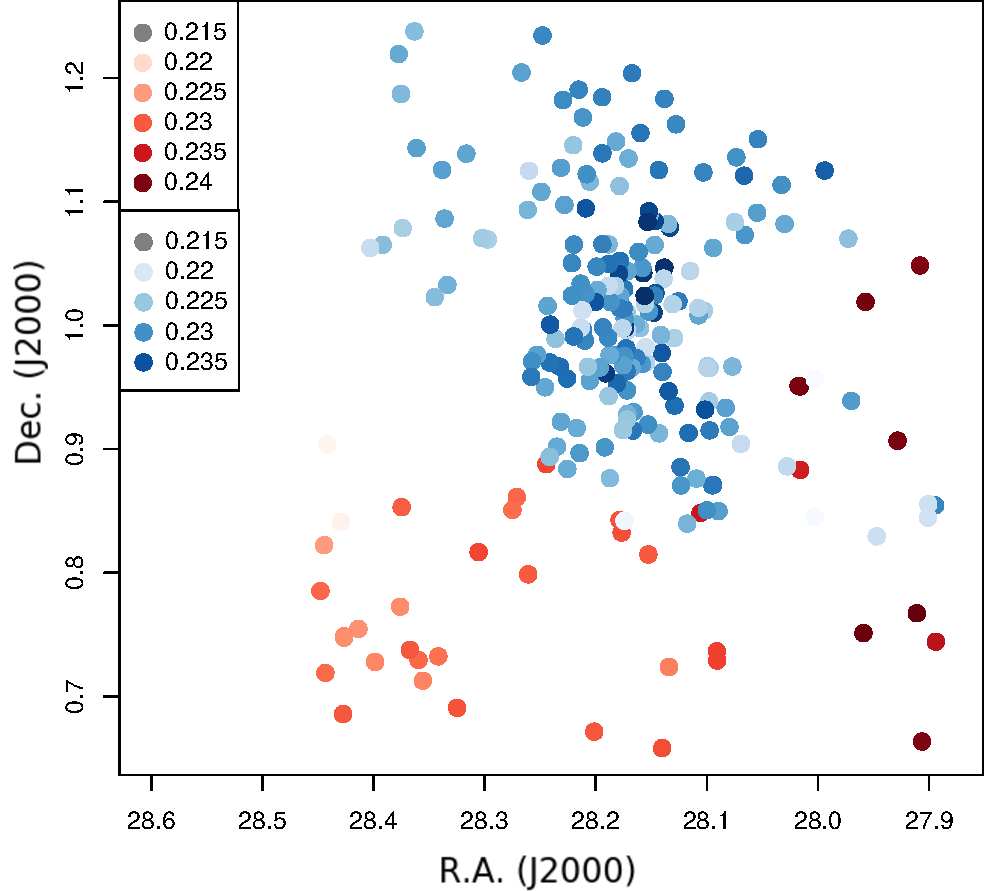
\includegraphics[scale=0.25]{redshift_angular.pdf}
 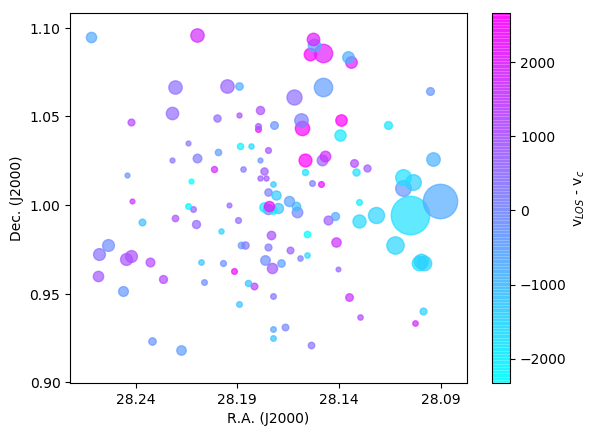
\includegraphics[scale=0.35]{dstest_a267_1.png}
 % redshift_angular.pdf: 0x0 px, 300dpi, 0.00x0.00 cm, bb=
\end{figure}
}
\frame{
\begin{figure}[ht!]
 \centering
 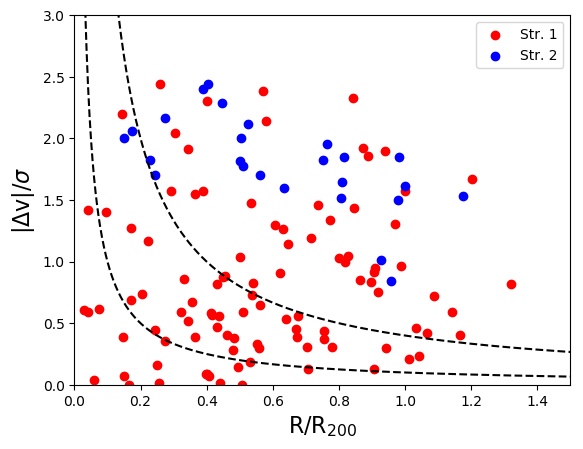
\includegraphics[scale=0.3]{a267_phasespace.png}
 \includegraphics[scale=0.17]{fig_results2.eps}
 % a267_phasespace.png: 583x449 px, 100dpi, 14.81x11.40 cm, bb=0 0 420 323
\end{figure}

}
\subsection{Statistical analysis of the magnetic fields in merging clusters.}
\frame{
\begin{figure}[ht!]
 \centering
 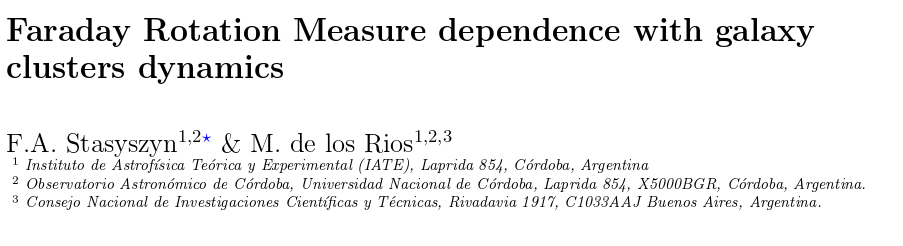
\includegraphics[scale=0.6]{magnetic_paper.png}
 % magnetic_paper.png: 710x230 px, 96dpi, 18.78x6.08 cm, bb=0 0 532 172
\end{figure}
}

\frame{
\begin{figure}[ht!]
 \centering
 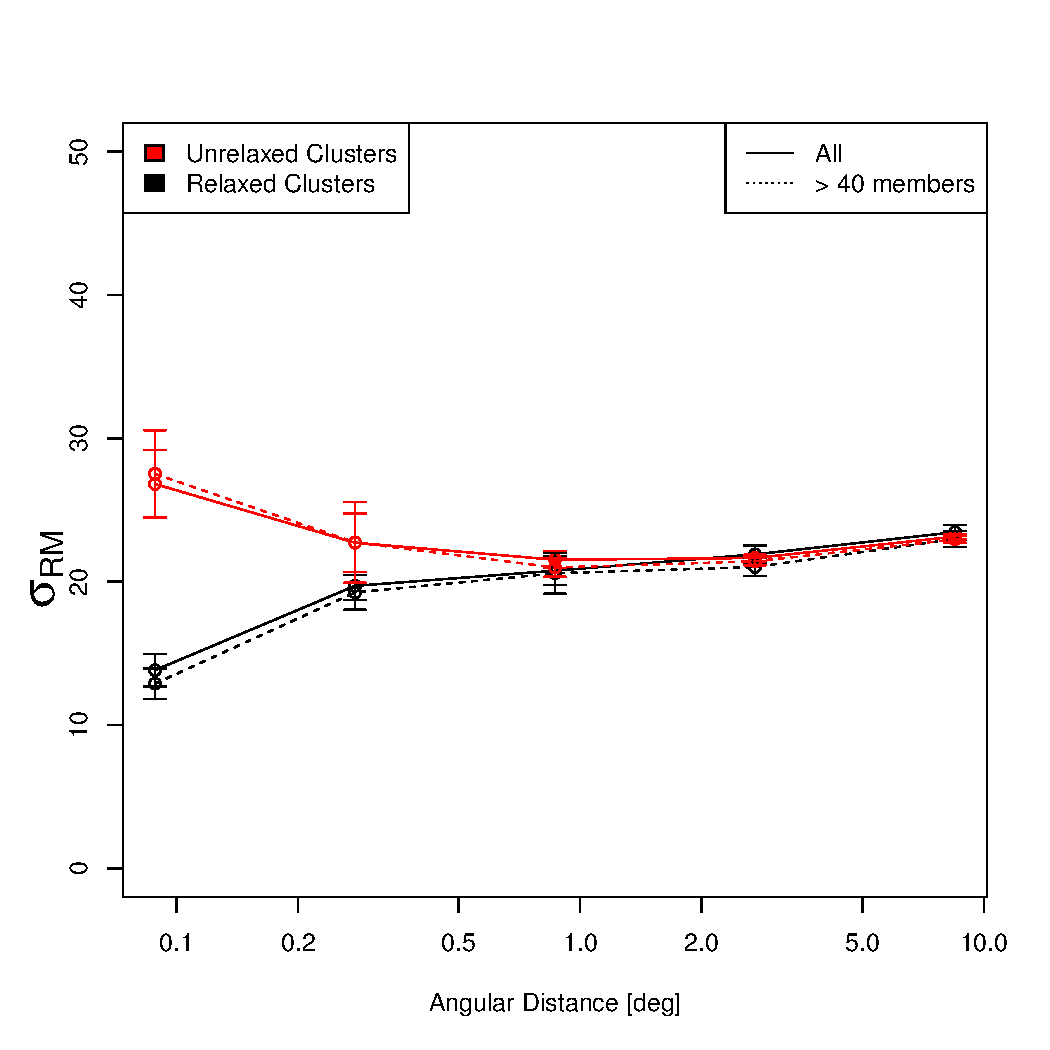
\includegraphics[scale=0.28]{AngTay01.pdf}
 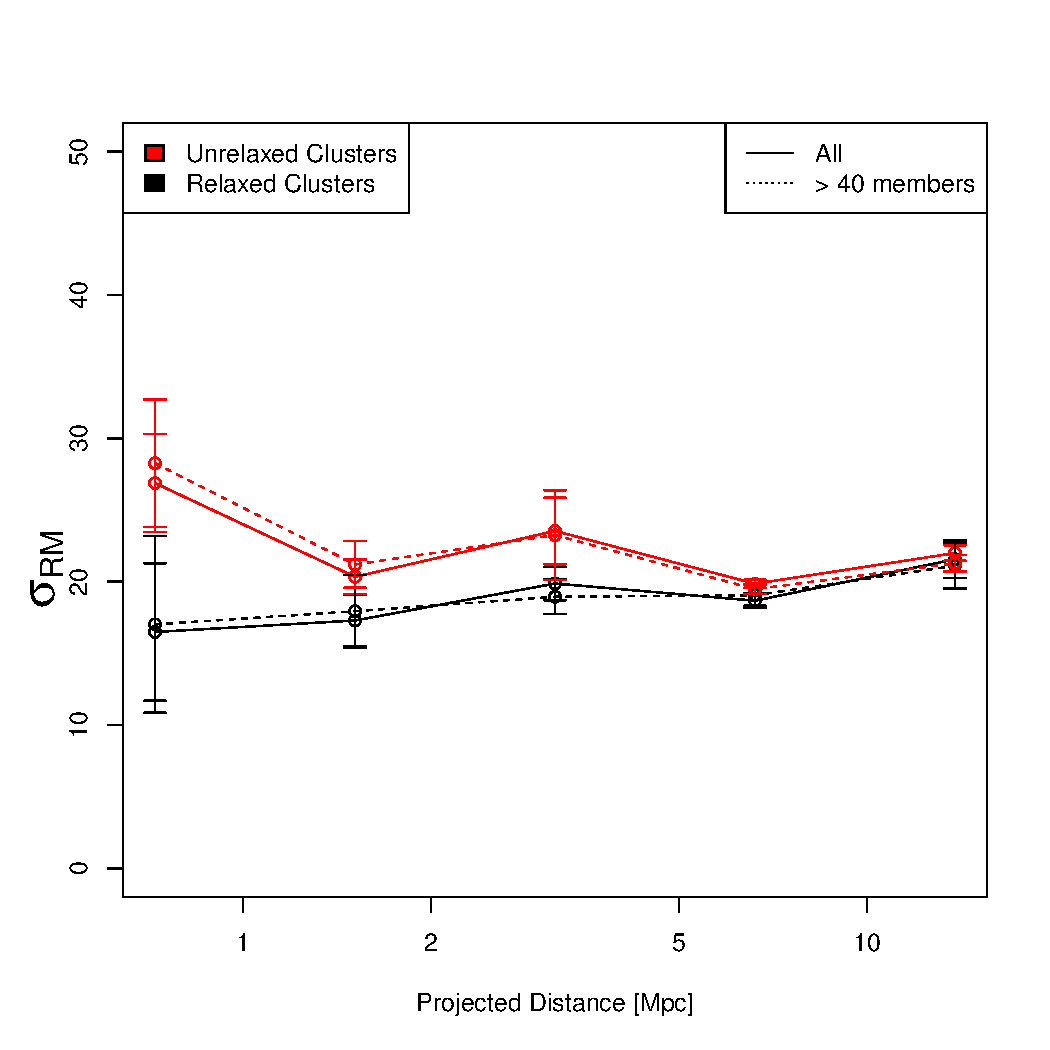
\includegraphics[scale=0.28]{ProTay01.pdf}
 % AngTay01.pdf: 0x0 px, 300dpi, 0.00x0.00 cm, bb=
\end{figure}

}
\section{\texttt{CosmoMl}:Machine Learning techniques applied to the CMB.}

\frame{
\tableofcontents[ 
    currentsubsection, 
    sectionstyle=show/hide, 
    sectionstyle=show/shaded, 
    ] 
}

\subsection{Construction of the data set.}
\subsection{Unsupervised methods.}
\subsection{Supervised methods.}
\subsection{Cosmological parameters Angular distributions.}

\section{Conclusions.}

\frame{
\tableofcontents[ 
    currentsubsection, 
    sectionstyle=show/hide, 
    sectionstyle=show/shaded, 
    ] 
}


\frame{
\begin{figure}[ht!]
 \centering
 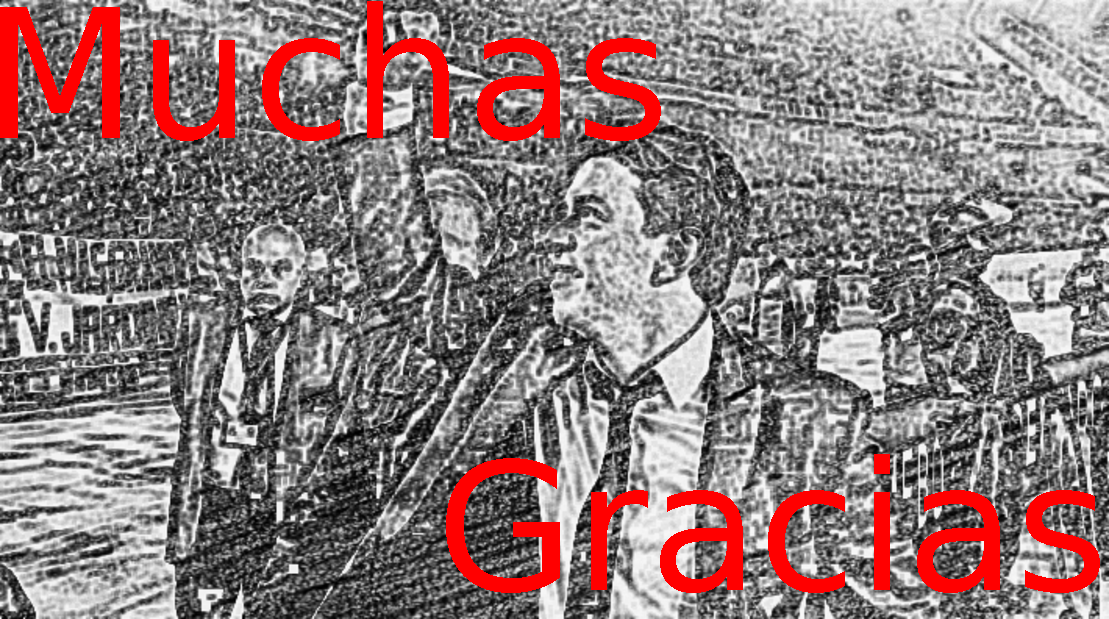
\includegraphics[scale=0.63]{./gracias2.pdf}
% nfw_velocity_distributions.pdf: 0x0 pixel, 300dpi, 0.00x0.00 cm, bb=
\end{figure}
}
\end{document}

